\documentclass{beamer}

\usetheme{Warsaw}
\usecolortheme{crane}

\usepackage{courier}
\usepackage[utf8]{inputenc}
\usepackage{ngerman}
\usepackage{pgf}
\usepackage{amsmath}
\usepackage{hyperref}
\usepackage{listings}
\usepackage{color}
\usepackage{ulem}

\definecolor{dkgreen}{rgb}{0,0.6,0}
\definecolor{gray}{rgb}{0.5,0.5,0.5}
\definecolor{mauve}{rgb}{0.58,0,0.82}

\lstset{frame=tb,
  language=Python,
  aboveskip=3mm,
  belowskip=3mm,
  showstringspaces=false,
  columns=flexible,
  basicstyle={\footnotesize\ttfamily},%{\tiny\ttfamily},
  numbers=none,
  numberstyle=\tiny\color{gray},
  keywordstyle=\color{blue},
  commentstyle=\color{dkgreen},
  stringstyle=\color{mauve},
  breaklines=true,
  breakatwhitespace=true
  tabsize=3
}

\setbeamercolor{frametitle}{fg=black}
\setbeamercolor{title}{fg=black}
\setbeamercolor{block title}{fg=blue}
\setbeamercolor{item}{fg=black,bg=white}

\logo{
\includegraphics[height=1.3cm]{pics/logo}} 
\newcommand{\linklogo}{
\includegraphics[width=0.3cm]{pics/link}}

\newcommand{\mytilde}{\raise.17ex\hbox{$\scriptstyle\mathtt{\sim}$}}

\begin{document}

\title{cp-logic}
\subtitle{Umsetzung der Konzepte aus der Vorlesung \\
\textit{Diskrete Mathematik und Logik} \\
in eine Toolbox fur Studierende (Bachelorarbeit)}
\author{Adrianus Kleemans}
\date{22.05.2014}

\frame{\titlepage} 

\frame{
\frametitle{Inhaltsverzeichnis}\tableofcontents[hideothersubsections]} 

\section{Einleitung}
\subsection{GUI}
\frame{
\frametitle{GUI der Toolbox}
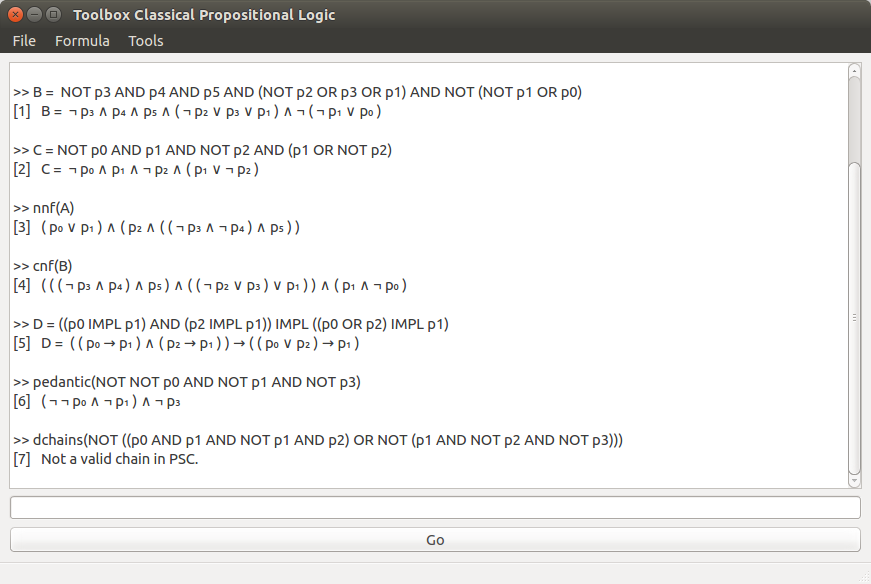
\includegraphics[width=0.85\linewidth]{pics/window}
}

\subsection{Motivation}
\frame{
\frametitle{Motivation}
Ausgangspunkt: Skript \textbf{Diskrete Mathematik und Logik} \\
Im Skript werden viele Algorithmen beschrieben:
\begin{figure}
\centering
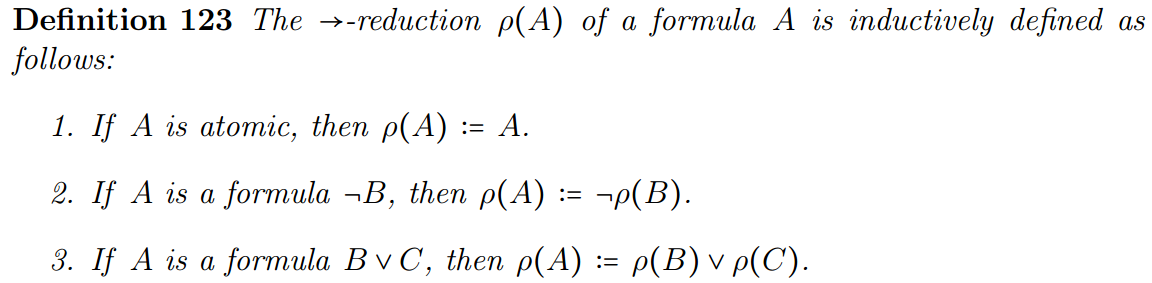
\includegraphics[width=.85\linewidth]{pics/script}
\end{figure}
Ideen:
\begin{itemize}
\item Lernprozess durch Ausprobieren
\item Schnelles Feedback über Korrektheit
\end{itemize}
}

\subsection{Anforderungen}
\frame{
\frametitle{Anforderungen an das Endprodukt}
\begin{itemize}
\item Nähe zum Skript (gleiche Namen und Funktionen)
\item Abbildung aller in der Vorlesung gewichteten Teile des Skripts
\item Detaillierte Fehlerbehandlung, ``fail safe''
\item Graphische Darstellung (z.B. der Deduktionsketten)
\item Einfache Eingabemöglichkeit für Benutzer
\item Nachvollziehbarkeit (History, gespeicherte Formeln)
\item Laden von Formeln aus Dateien
\end{itemize}
}

\frame{
\frametitle{Anforderungen an die Technologie}
Diverse Anforderungen, welche die Möglichkeiten einschränkten:
\begin{itemize}
\item Unicode-Unterstützung ($\vee$, $\wedge$, $\neg$, $\top$, ...)
\item Geeignete Datenstrukturen (verschachtelte Listen, assoziative Arrays, binäre Bäume)
\item Unabhängigkeit vom Betriebssystem
\item Lesbarer Code, offen für Erweiterungen
\end{itemize}
}

\frame{
\frametitle{Verwendete Technologien}
Einige verwendete Technologien:
\begin{itemize}
\item Programmiersprache: Python
\item GUI: QT4 (\texttt{pyside}), \texttt{pygame}
\item Versionsverwaltung: git
\item Unit tests: Modul \texttt{unittest}
\item Unterstützende Technologien, z.B. \texttt{pyinstaller} zur Paketierung
\end{itemize}
}

\subsection{Methoden}
\frame{
\frametitle{Methoden}
Entwicklung mit einigen recht intuitiven Methoden:
\begin{itemize}
\item TDD (Test Driven Development): Unit Tests
\item Orientierung der Tests an Use cases (direkt aus Skript und Übungen)
\item Grundklasse: \texttt{Formula}, andere Klassen bauen darauf auf
\item Interaktive Erarbeitung, Feedback der Betreuer
\end{itemize}
}

\begin{frame}[fragile]
\frametitle{Test Driven Development}
Zuerst die Spezifikation des Testfalls:
\begin{lstlisting}
def test_invalidFormula_propositions(self):
    try: f = Formula('p0 OR OR NOT p1')
    except FormulaInvalidError: pass
    else: self.fail("Connectives without propositions are not allowed.")
\end{lstlisting}
Danach in der Formel-Klasse umsetzen, bis der Testfall erfolgreich durchläuft.
$\Rightarrow$ Auch später noch Nutzen der Tests als Regressionstests!
\end{frame}

\subsection{Resultat}
\frame{
\frametitle{Ein paar Kennzahlen}
Ein paar Kennzahlen:
\begin{itemize}
\item 8 Klassen mit insgesamt \mytilde 2000 Zeilen Code
\item 35 Seiten Bericht + zusätzliche Dokumentation im Code für \mytilde 70 Funktionen
\item insgesamt \mytilde 120 Tests, ein Grossteil für die Formel-Klasse
\item allermeisten Anforderungen wurden umgesetzt
\end{itemize}
}

\frame{
\frametitle{Klassen-Aufteilung}
\begin{figure}
\centering
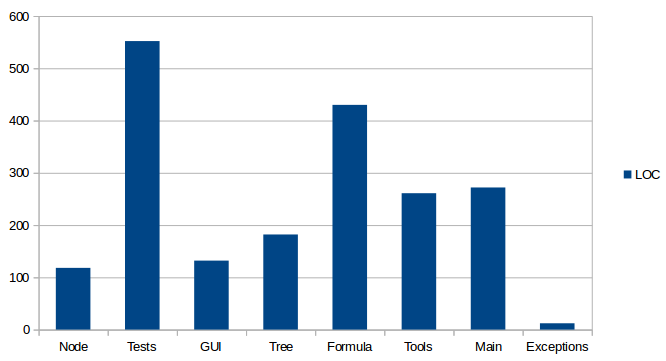
\includegraphics[width=0.9\linewidth]{pics/classes2}
\end{figure}
}

\section{Aufbau}
\subsection{UML}
\frame{
\frametitle{Aufbau (UML) I}
\begin{figure}
\centering
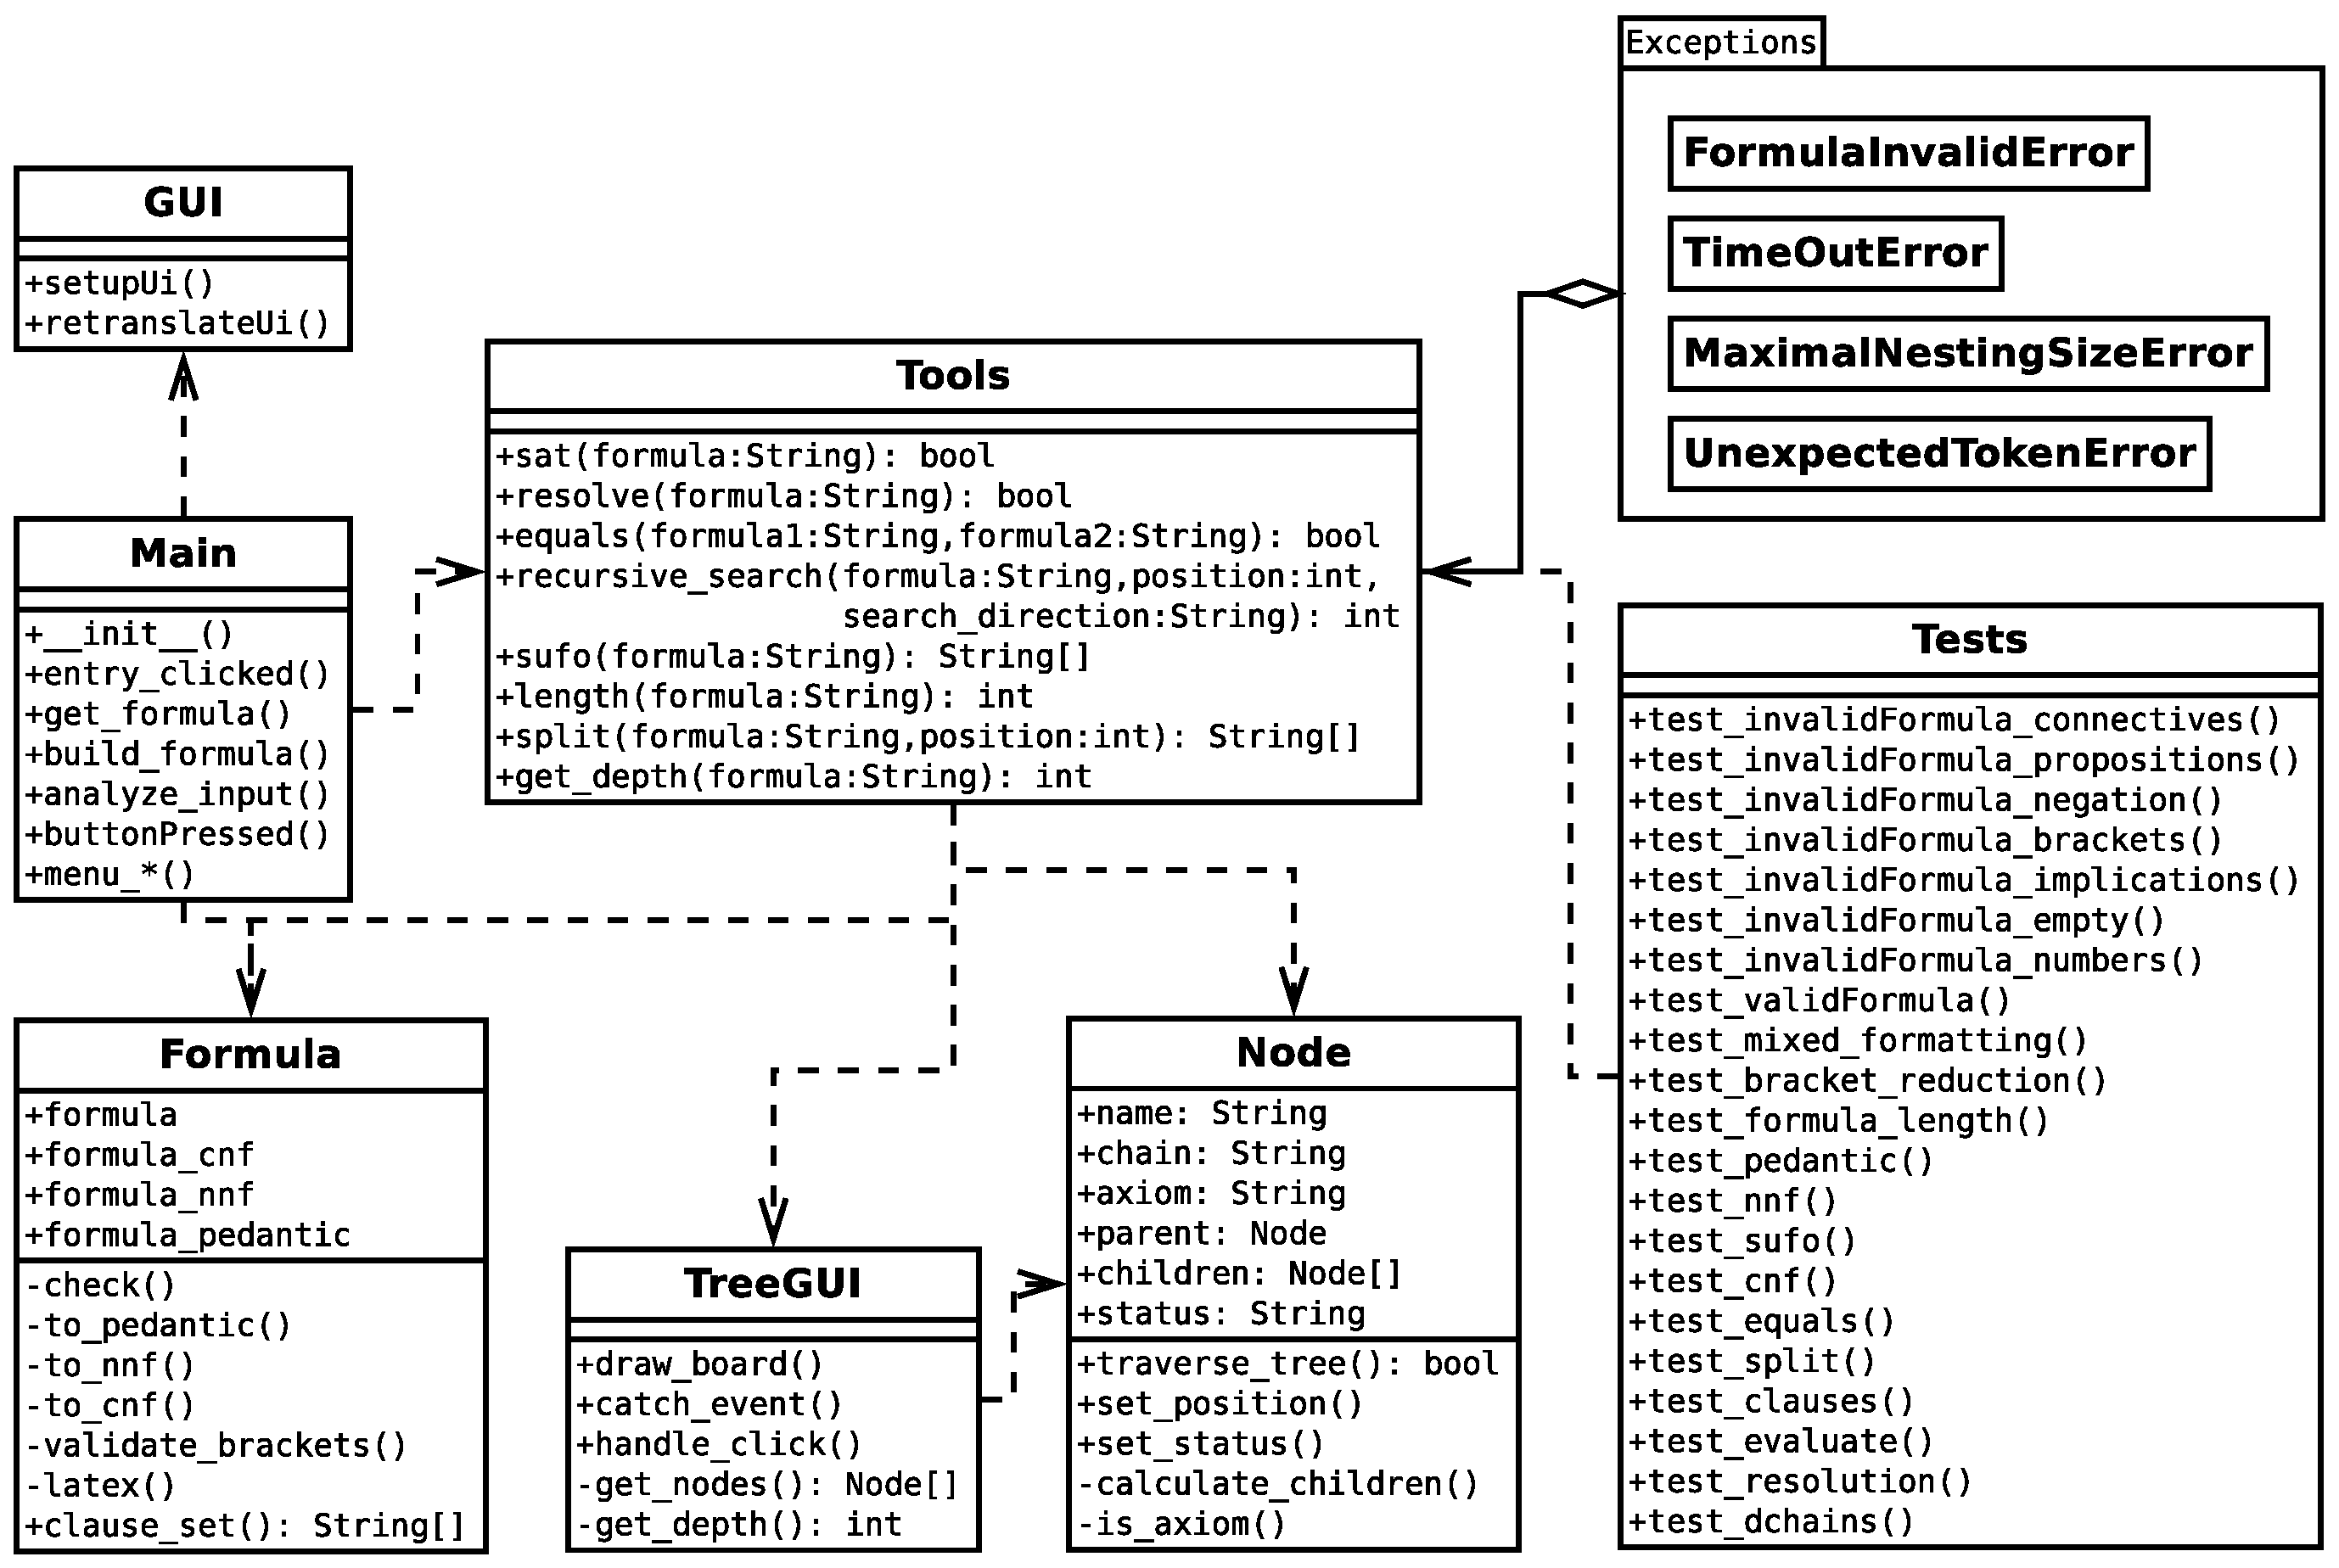
\includegraphics[width=0.8\linewidth]{pics/UML_complete}
\end{figure}
}

\frame{
\frametitle{Aufbau (UML) II}
\begin{figure}
\centering
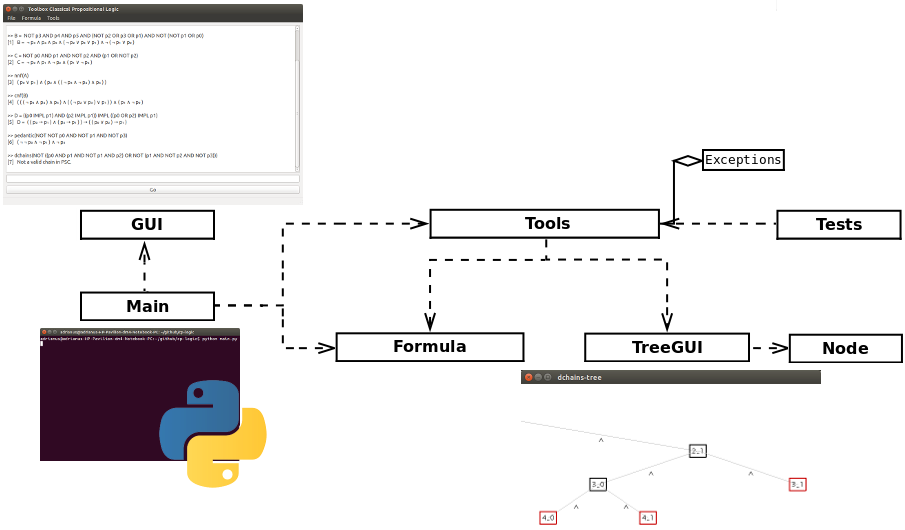
\includegraphics[width=0.9\linewidth]{pics/UML2}
\end{figure}
}

\frame{
\frametitle{Klassen}
\begin{itemize}
\item \textbf{Main} - Einstiegspunkt
\item \textbf{GUI} - Python/QT4-Benutzeroberfläche (Fenster mit Menü)
\item \textbf{Formula} - Formel (mit Normalformen, Sufos, etc.) 
\item \textbf{Tools} - Weiterführende Funktionen (Erfüllbarkeit, Klauselmengen, lineare Suche, Tiefensuche etc.)
\item \textbf{TreeGUI} - Deduktionsketten-Baum (Darstellung)
\item \textbf{Node} - Deduktionsketten-Knoten (rekursiv berechnet)
\item \textbf{Exceptions} - eigene Fehlerbehandlung
\item \textbf{Tests} - Funktionale Tests, Regressionstests
\end{itemize}
}

\subsection{Normalformen}
\frame{
\frametitle{Normalformen}
Basisformel $A = p_1 \vee p_2 \rightarrow \top$.
\begin{itemize}
\item pedantic(): Hierarchische Struktur: $\neg$ vor $\vee\,\wedge$ vor $\to$
\begin{align*}
pedantic(A) =  ( p_1 \vee p_2 ) \rightarrow \top
\end{align*}
\item nnf(): \sout{Implikationen}, Negationen nur vor atomaren Prop.
\begin{align*}
nnf(A) = ( \neg p_1 \wedge \neg p_2 ) \vee \top
\end{align*}
\item cnf(): Konstanten ersetzen, \footnotesize{$p_1 \vee (p_2 \wedge p_3) \to (p_1 \vee p_2) \wedge (p_1 \vee p_3)$}
\normalsize
\begin{align*}
cnf(A) = ( \neg p_1 \vee ( p_0 \vee \neg p_0 ) ) \wedge ( \neg p_2 \vee ( p_0 \vee \neg p_0 ) )
\end{align*}
\end{itemize}
}

\frame{
\frametitle{Übersicht Abhängigkeiten Normalformen}
\begin{figure}
\centering
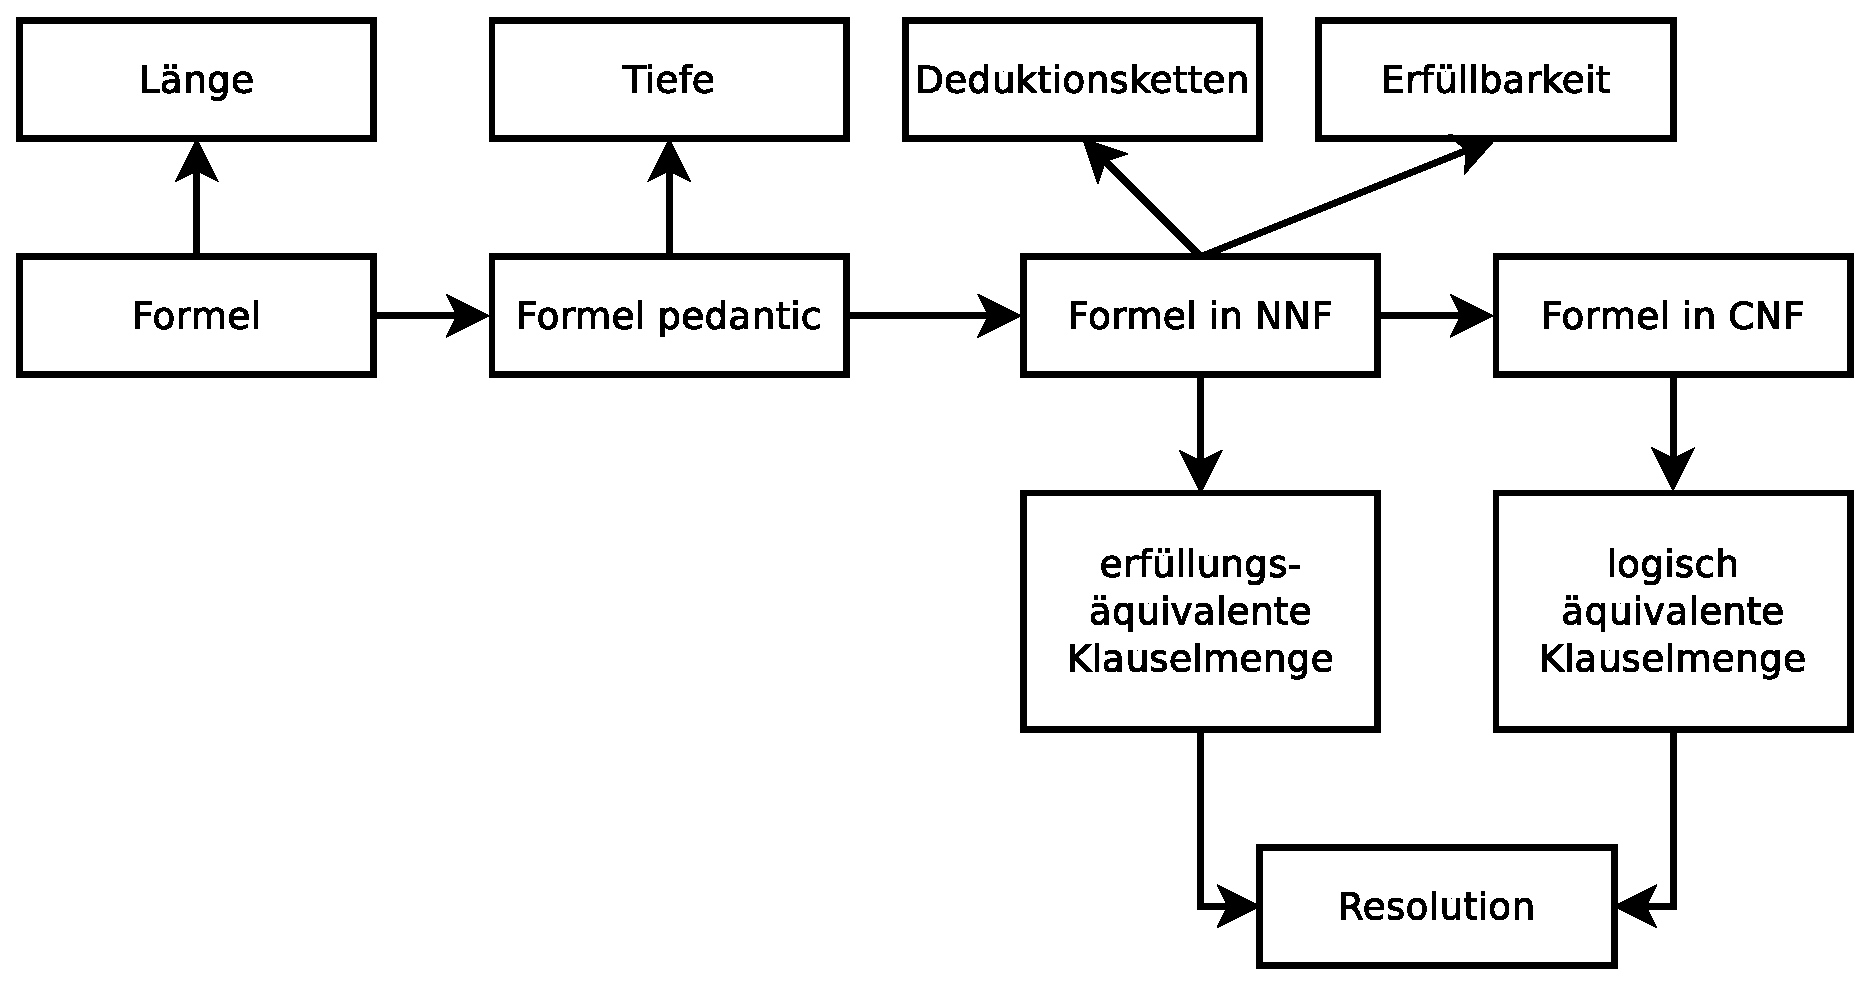
\includegraphics[width=1\linewidth]{pics/Normalformen}
\end{figure}
}

\subsection{Formel-Objekte}
\frame{
\frametitle{Modellierung Formel-Klasse I}
2 Ideen: Entweder die einzelnen Normalformen als einzelne Objekte abbilden...
\begin{figure}
\centering
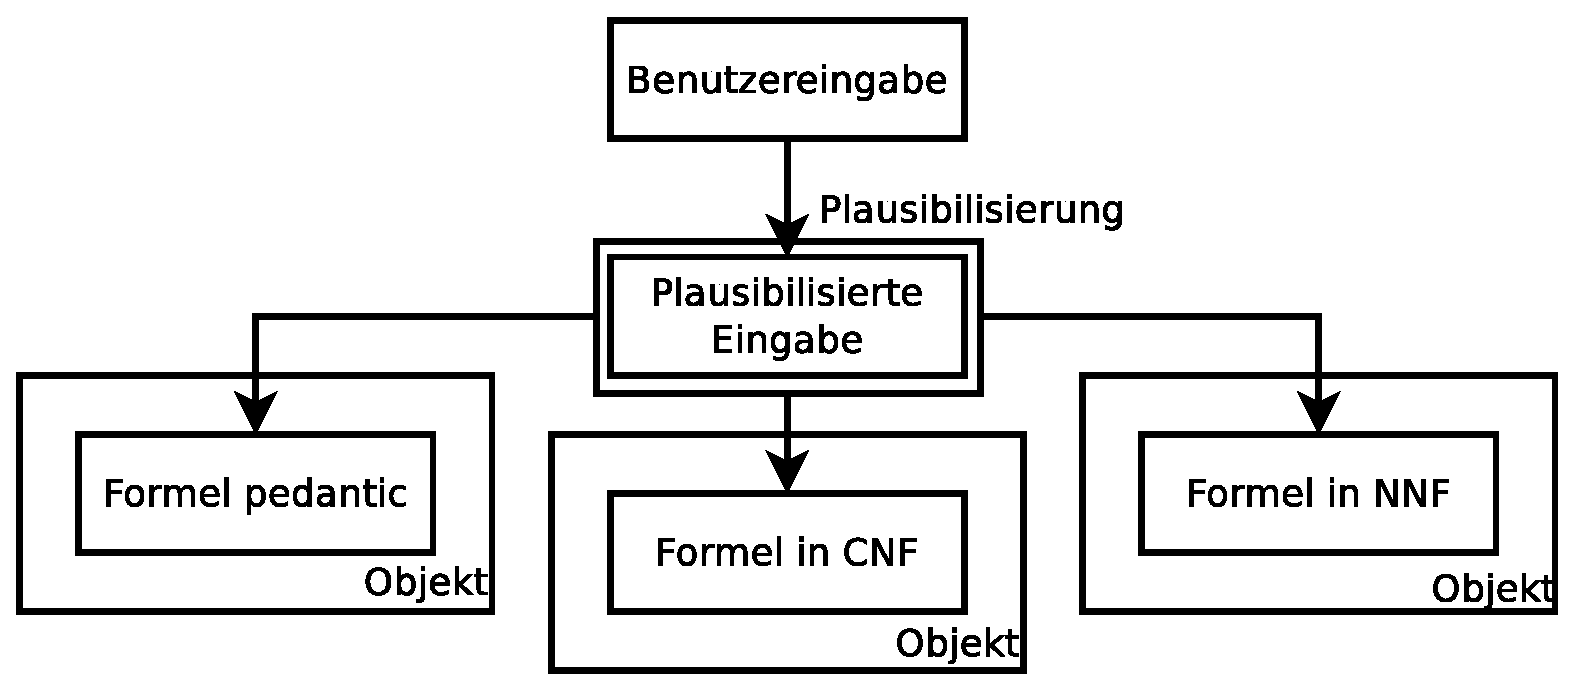
\includegraphics[width=.8\linewidth]{pics/Konzept_Formel2}
\end{figure}
}

\frame{
\frametitle{Modellierung Formel-Klasse II}
...oder Formel mit Normalformen als einzelnes Objekt abbilden.
\begin{figure}
\centering
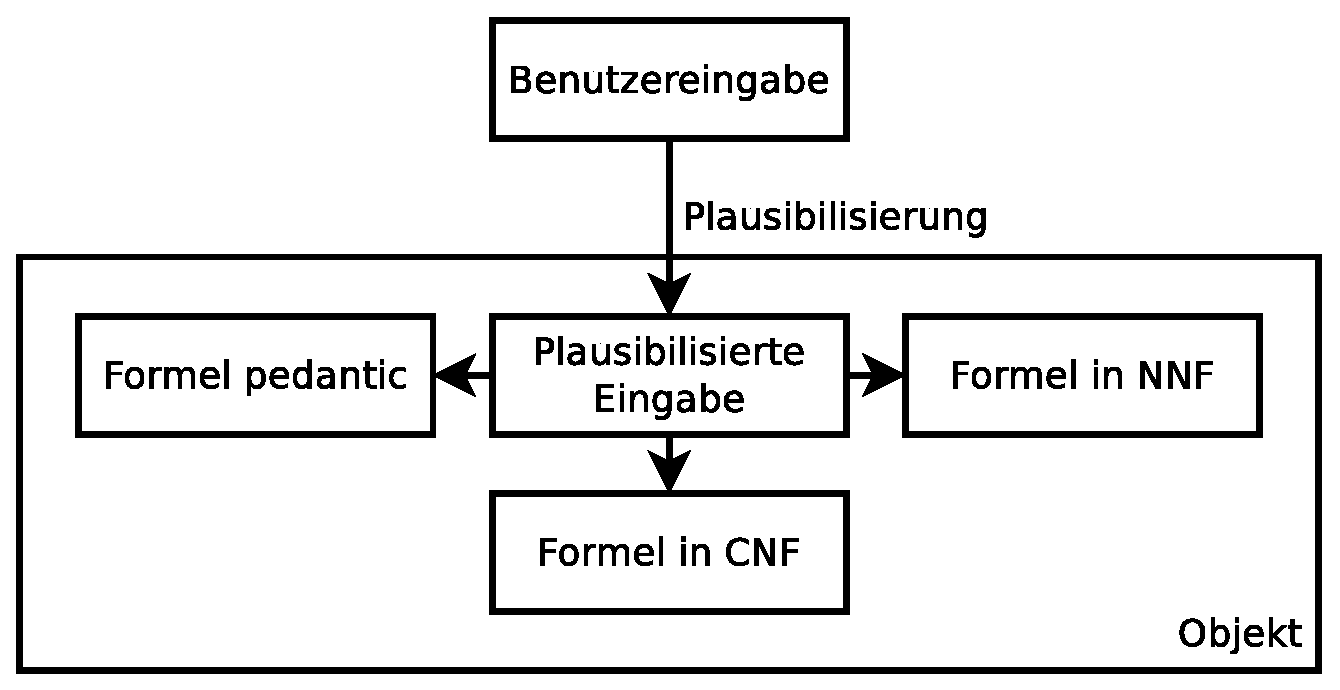
\includegraphics[width=.7\linewidth]{pics/Konzept_Formel}
\end{figure}
$\Rightarrow$ Beide Ansätze Vor- und Nachteile. \\
In meinem Konzept zweiter Vorschlag sinnvoller (Metavar.)
}

\subsection{Funktionsübersicht}
\frame{
\frametitle{Funktionsübersicht}
Die wichtigsten Funktionen:
\begin{itemize}
\item nnf(), cnf(), pedantic() - Normalformen
\item length() - Länge
\item sufo() - Subformulas
\item sat() - Test auf Erfüllbarkeit
\item clause\_set() - Klauselmengen
\item evaluate() - Evaluiert Formeln auf Wahrheitswert
\item resolution() - Resolution
\item dchains() - Deduktionsketten
\end{itemize}
}

\subsection{Fehlermeldungen}
\frame{
\frametitle{Fehlermeldungen}
Katalog von Fehlermeldungen zur Hilfe des Benutzers:
\begin{itemize}
\item Ungültige Zeichen: $p_0 a$
\item Proposition ohne Index: $p$
\item Nicht verknüpfte Propositionen: $p_0 p_1$
\item Alleinstehende Indizes oder Negation: $p_0 \vee {}_2$ oder $p_0 \vee \neg$
\item Ungültige Konjunktion: $p_0 \wedge \vee p_1$
\item Gemischte $\wedge$ und $\vee$ auf selber Ebene: $p_0 \wedge p_1 \vee p_2$
\item Ungültige Implikation: $\rightarrow p_0$ oder $p_0 \rightarrow p_1 \rightarrow p_2$
\item Ungültige Klammernsetzung: $((p_0 \wedge p_1) \vee p_2$
\item ...
\end{itemize}
}

\section{Algorithmen}
\subsection{Verarbeitung Benutzereingabe}
\frame{
\frametitle{Benutzereingabe}
Verarbeitung der Eingabe durch Benutzer:
\begin{figure}
\centering
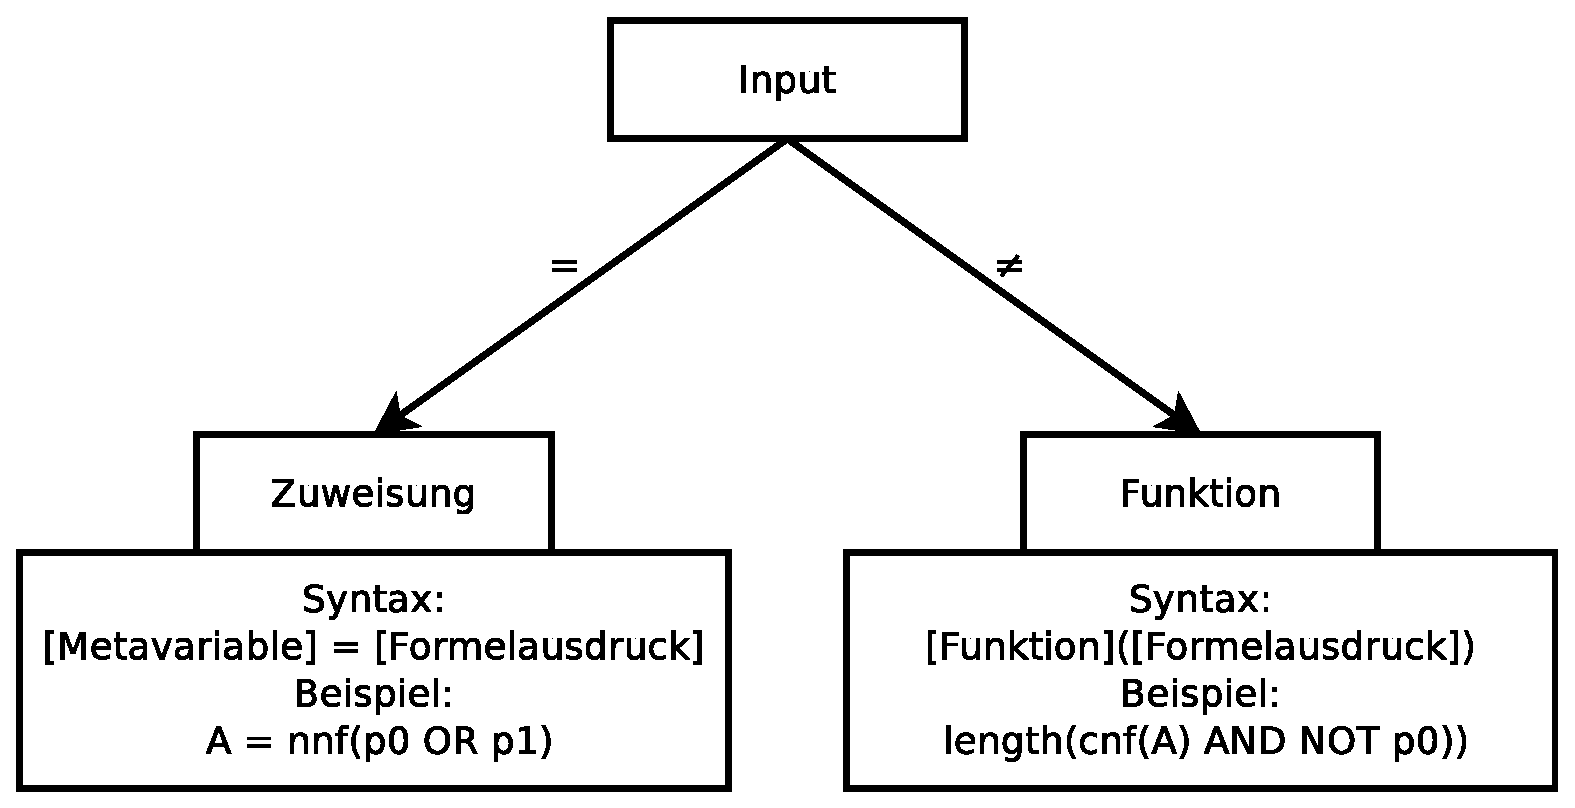
\includegraphics[width=.82\linewidth]{pics/input}
\end{figure}
}

\subsection{Suche in Formeln}
\frame{
\frametitle{Suche in Formeln}
Als Beispiel für die Auflösung von Negationen (NNF) müssen zusammengehörige Klammernpaare identifiziert werden.
\begin{figure}
\centering
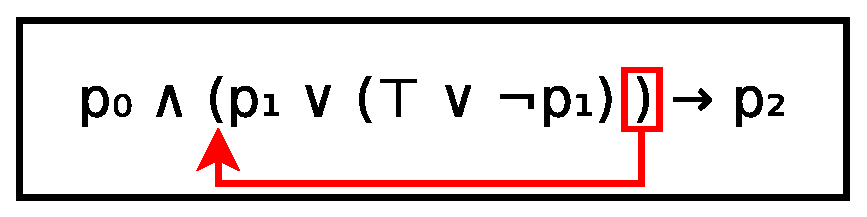
\includegraphics[width=.5\linewidth]{pics/linear_search}
\end{figure}
$\Rightarrow$ Einfachste Möglichkeit, die zugehörige Klammer zu finden?
}

\frame{
\frametitle{Konzept Formeltiefe}
Einführung des Konzepts der \textbf{Tiefe}. Zerlegung einer Formel
\begin{align*}
p_0 \wedge ( \neg p_1 \vee ( p_2 \wedge \neg p_3 ) \vee ( p_1 \wedge ( \top \vee p_3 ) ) )
\end{align*}
in verschiedene Ebenen:
\begin{figure}
\centering
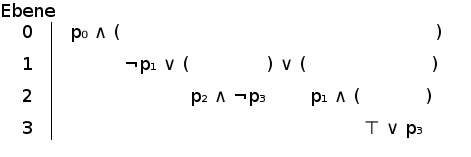
\includegraphics[width=.6\linewidth]{pics/levels}
\end{figure}
}

\subsection{Satisfiability}
\frame{
\frametitle{Satisfiability}
Pseudocode:
\begin{enumerate}
\item Wandle Formel in NNF um
\item Sammle Anzahl $n$ atomare Propositionen
\item Für alle $2^n$ Valuationen, tue folgendes:
  \begin{enumerate}
  \item Setze Valuation an Stelle der Propositionen ein
  \item Evaluiere den Wahrheitswert und reduziere diesen auf \texttt{true} oder \texttt{false}
  \item Falls \texttt{true}, beende und gib diese Valuation aus.
  \end{enumerate}
\end{enumerate}

Auflösung durch \texttt{evaluate()}, z.B.:
\begin{align*}
\bot \vee &( \bot \wedge \top ) \\
\bot &\vee \bot \\
&\bot
\end{align*}
}

\subsection{Klammern reduzieren}
\frame{
\frametitle{Klammern setzen}
Formeln für Meta-Veriablen können nicht 1:1 eingesetzt werden:
\begin{align*}
&>> A = p_0 \wedge \neg p_1\\
&>> \neg A \\
&[0] \textcolor{red}{\neg p_0 \wedge \neg p_1}
\end{align*}
Zusätzliches Einfügen von Klammern entschärft dies:
\begin{align*}
&>> \neg A \\
&[0] \textcolor{green}{\neg (p_0 \wedge \neg p_1)}
\end{align*}
Problem: Aufruf interner Funktionen verändert Formel!
\begin{align*}
(p_0 \wedge \neg p_1), ((p_0 \wedge \neg p_1)), (((p_0 \wedge \neg p_1))), ...
\end{align*}
}

\frame{
\frametitle{Klammern reduzieren}
Es wird ein Verfahren benötigt, um Klammern zu reduzieren. \\
$\Rightarrow$ Festhalten der Ebenenübergänge. Wird eine Ebene auf beiden Seiten ``übersprungen'', ist der Übergang unnötig.
\begin{align*}
p_0 \vee \underbrace{(}_{0-1} \underbrace{\textcolor{red}{(}}_{1-2} p_1 \wedge \neg p_2 \underbrace{\textcolor{red}{)}}_{2-1} \underbrace{)}_{1-0}
\end{align*}
Findet dazwischen ein Übergang statt, werden Klammern benötigt:
\begin{align*}
p_0 \vee \underbrace{(}_{0-1} \underbrace{(}_{1-2} p_1 \wedge \neg p_2\underbrace{)}_{2-1} \vee \underbrace{(}_{1-2} p_0 \vee p_1 \underbrace{)}_{2-1} \underbrace{)}_{1-0}
\end{align*}

}

\section{Beispiele - Demo}
\subsection{Demo}
\frame{
\frametitle{Demo}
Einige Beispiele:
\begin{itemize}
\item Eingabe von Hand und per Datei - \texttt{sample\_file.formula}
\begin{itemize}
\item Formeln
\item Metavariablen
\item Verschachtelungen
\item Normalformen
\end{itemize}
\item Satisfiability
\item Deduktionsketten - \texttt{dchains.formula}
\end{itemize}
}

%\subsection{Deduktionsketten}
%\frame{
%\frametitle{Deduktionsketten}
%\begin{figure}
%\centering
%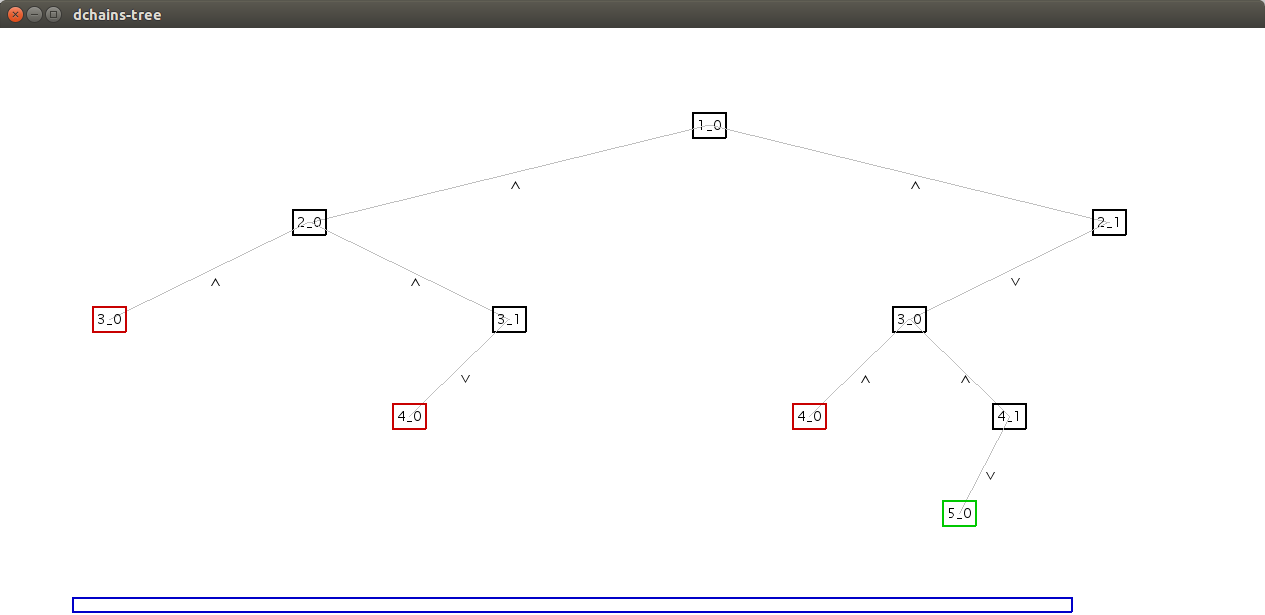
\includegraphics[width=1\linewidth]{pics/dchains}
%\end{figure}
%}

\section{Schluss}
\subsection{Herausforderungen}
\begin{frame}[fragile]
\frametitle{Herausforderungen I}
Vorsicht vor ``lazy evaluation'' (rekursive Knotenberechnung):
\begin{lstlisting}
def traverse():
  ...
  return ( child1.traverse() and child2.traverse() )
\end{lstlisting}
$\Rightarrow$ Baum wird nicht immer vollständig gezeichnet!
\begin{lstlisting}
def traverse():
  ...
  a = child1.traverse()
  b = child2.traverse()
  return ( a and b )
\end{lstlisting}
Mit Zwischenspeichern werden Zwischenschritte ausgeführt.
\end{frame}

\frame{
\frametitle{Herausforderungen II}
Komplexe Ausdrücke sollten evaluiert werden können: \\
\centering $>>$ \text{length(cnf(A AND p0 } $\wedge\, \neg\, p_3 \,$ \text{AND NOT B))}
\begin{itemize}
\item Auflösung von Metavariablen
\item Verknüpfung von Metavariablen, in Kombination mit Formeln
\item gemischter ASCII- und Unicode-Input
\item Pipeline von Funktionsaufrufen
\end{itemize}
$\Rightarrow$ Plausibilisierungen auf jeder Stufe
}

\frame{
\frametitle{Herausforderungen III}
Weitere Herausforderungen:
\begin{itemize}
\item ``Saubere'' und stabile Formel-Klasse als Basis
\item Eigene Entscheidungen ergänzend zum Skript (z.B. pedantic-Form)
\item Unicode-Unterstützung Linux/Windows
\item Skalierbares \& scrollbares Fenster für dchains
\end{itemize}
}


\subsection{Fazit}
\frame{
\frametitle{Fazit}
Fazit:
\begin{itemize}
\item Getestete, stabile Applikation mit graphischer Oberfläche
\item Sehr viel gelernt (Logik, Zusammenspiel Technologie, GUI)
\item Aufwand schwer abzuschätzen (z.B. Formel-Klasse)
\item Umgehen mit Anforderungen, Änderungen, Prioritäten
\end{itemize}
}

\subsection{Fragen} 
\frame{
\frametitle{Fragen?}
Fragen?
}

\end{document}